\documentclass[]{article}

\usepackage{listings}

\usepackage[a4paper, left=3cm, top=2cm, right=1cm, bottom=2cm]{geometry}
\usepackage[utf8]{inputenc}
\usepackage[english, russian]{babel}
% \usepackage{times}
\usepackage{verbatim}
\usepackage{hyperref}
\usepackage{graphicx}
\usepackage{caption}

\usepackage{float}



\captionsetup[figure]{name={Рисунок},labelsep=endash} 

\setlength{\parindent}{12.5mm} 
\pagestyle{empty}

\begin{document}
    
\newcommand{\student}{Заречный А.О.}


% настройки предмета
\newcommand{\lessonName}{Техниологии и инструментальные средства проектирования интеллектуальных систем}
\newcommand{\workName}{Разработка интеллектуальной системы}
\newcommand{\num}{3-4}
\newcommand{\teacher}{Кулеша В.И.}

% настройки работы
\newcommand{\purpose}{реализовать интеллектуальную систему.}
\newcommand{\task}{ 
    

    \begin{enumerate}

    \item Выбрать средства для реализации системы.
    \item Реализовать интеллектуальную систему.
    \item Загрузить данные в систему.
    
    \end{enumerate}

}

\newcommand{\result}{
    Предметная область --- менеджер паролей.




    \begin{enumerate}
        \item {
        
            Для реализации выбранной предметной области выбраны следующие средства:
            \begin{itemize}
                \item для серверной части был выбран Python с библиотекой FastAPI для поддержки запросов;
                \item для клиентской части был выбран фреймворк Flutter для разработки кроссплатформенного приложения.
            \end{itemize}
            
        }    

        \item {
            С учетом выбранных средства была реализована интеллектуальная система. Исходный код:
            \begin{figure}[H]
                \centering
                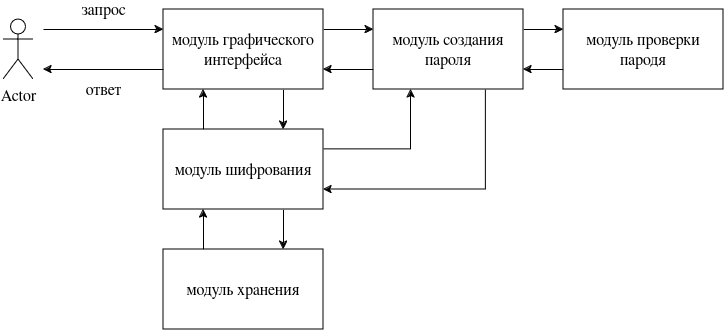
\includegraphics[width=\textwidth]{assets/shema.png}
                \caption{QR-код с ссылкой на исходный код}
            \end{figure}
        }
        

        \item {
            В приложение были загружены следующие данные:
            \begin{figure}[H]
                \centering
                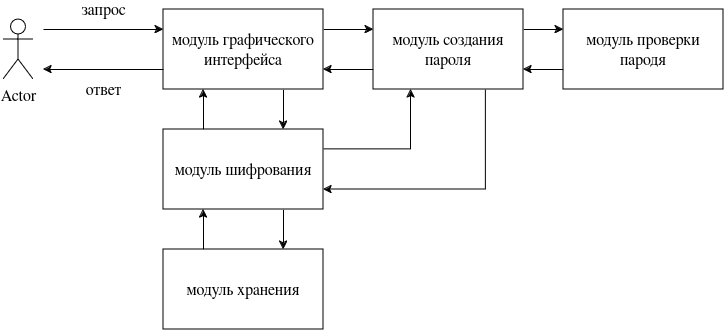
\includegraphics[width=\textwidth]{assets/shema.png}
                \caption{QR-код с ссылкой на исходный код}
            \end{figure}
        }
    \end{enumerate}

}
\newcommand{\conclusion}{
    реализовали интеллектуальную систему.
}

    \fontsize{14}{17.5}\selectfont    
    \begin{center}
        МИНИСТЕРСТВО ОБРАЗОВАНИЯ РЕСПУБЛИКИ БЕЛАРУСЬ \\
        УЧРЕЖДЕНИЕ ОБРАЗОВАНИЯ \\
        <<БРЕСТСКИЙ ГОСУДАРСТВЕННЫЙ ТЕХНИЧЕСКИЙ УНИВЕРСИТЕТ>> \\
        ФАКУЛЬТЕТ ЭЛЕКТРОННО-ИНФОРМАЦИОННЫХ СИСТЕМ \\
        Кафедра интеллектуальных информационных технологий \\[6cm]

        Отчет \\
        по дисциплине \\
        <<\lessonName>> \\
        по лабораторной работе № \num \\
        <<\workName>> \\[5cm]
    \end{center}

    \begin{flushright}
        \begin{minipage}{0.25\textwidth}
            \begin{flushleft}
                Выполнил: \\
                студент 4 курса \\
                группы ИИ-22 \\
                \student \\
                Проверил: \\
                \teacher
            \end{flushleft}
        \end{minipage}
    \end{flushright}

    \vfill 

	\begin{center}
		Брест \the\year
	\end{center}

    \newpage
    {\bfseries Цель:} \purpose 

    {\bfseries Постановка задачи:} \task

    {\bfseries Ход работы: }

    \result
    {\bfseries Вывод: }\conclusion

\end{document}